\documentclass{standalone}
\usepackage{tikz}
\usetikzlibrary{patterns, positioning}

\begin{document}
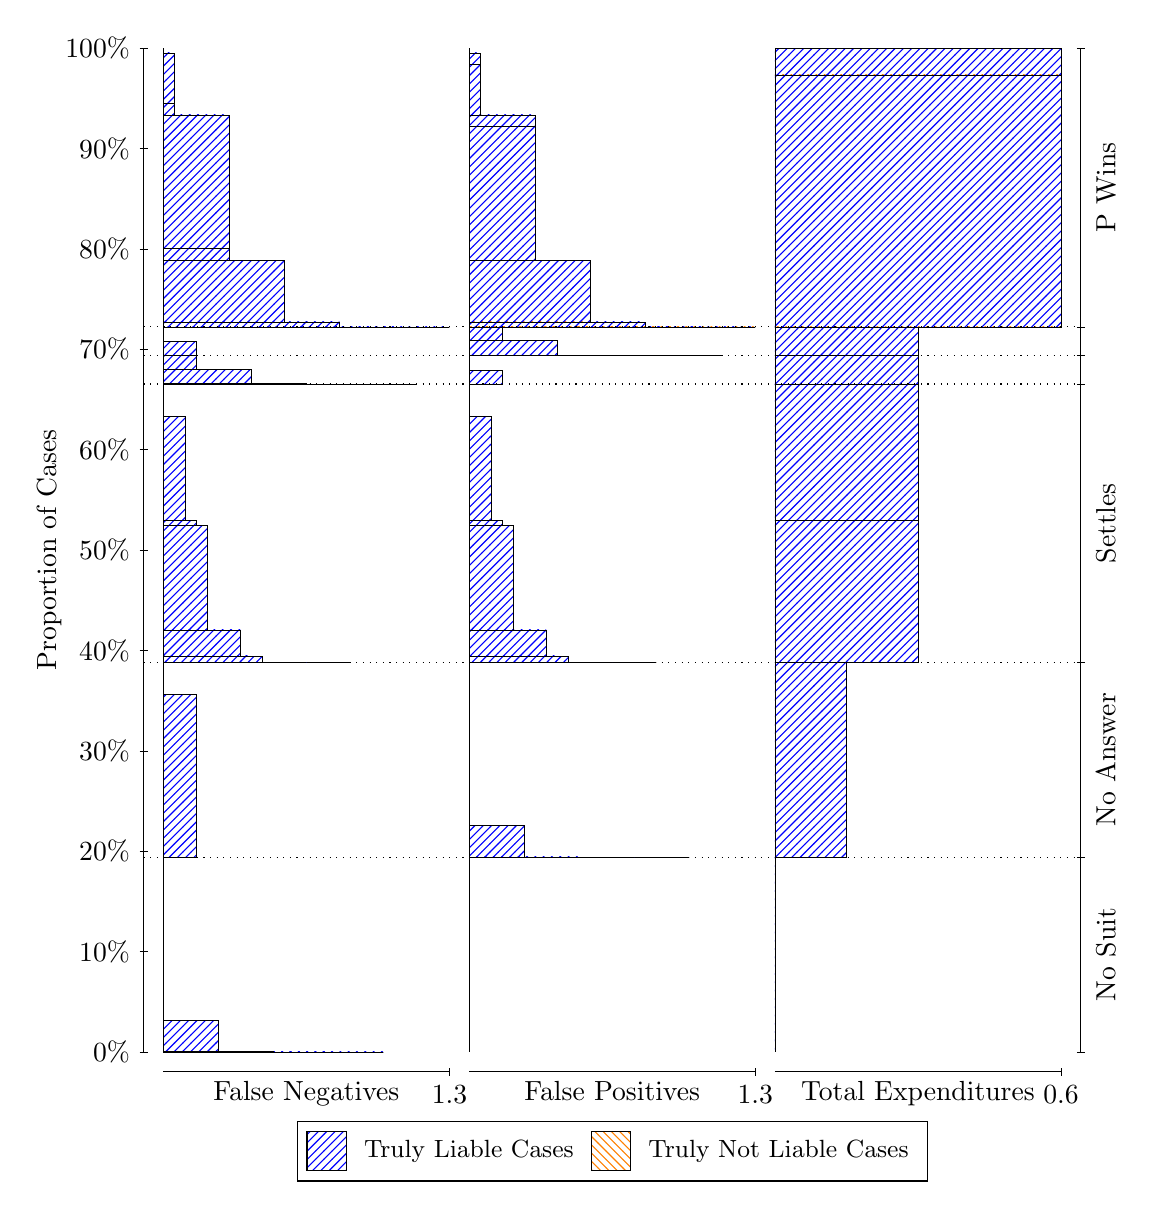
\begin{tikzpicture}
\draw[black, very thin] (1.5,1.75) -- (1.5,14.5);
\node[rotate=90, anchor=center] at (0.3, 8.125) {Proportion of Cases};
\draw[black, very thin] (1.45,1.75) -- (1.55,1.75);
\node[anchor=east] at (1.45, 1.75) {0\%};
\draw[black, very thin] (1.45,3.025) -- (1.55,3.025);
\node[anchor=east] at (1.45, 3.025) {10\%};
\draw[black, very thin] (1.45,4.3) -- (1.55,4.3);
\node[anchor=east] at (1.45, 4.3) {20\%};
\draw[black, very thin] (1.45,5.575) -- (1.55,5.575);
\node[anchor=east] at (1.45, 5.575) {30\%};
\draw[black, very thin] (1.45,6.85) -- (1.55,6.85);
\node[anchor=east] at (1.45, 6.85) {40\%};
\draw[black, very thin] (1.45,8.125) -- (1.55,8.125);
\node[anchor=east] at (1.45, 8.125) {50\%};
\draw[black, very thin] (1.45,9.4) -- (1.55,9.4);
\node[anchor=east] at (1.45, 9.4) {60\%};
\draw[black, very thin] (1.45,10.675) -- (1.55,10.675);
\node[anchor=east] at (1.45, 10.675) {70\%};
\draw[black, very thin] (1.45,11.95) -- (1.55,11.95);
\node[anchor=east] at (1.45, 11.95) {80\%};
\draw[black, very thin] (1.45,13.225) -- (1.55,13.225);
\node[anchor=east] at (1.45, 13.225) {90\%};
\draw[black, very thin] (1.45,14.5) -- (1.55,14.5);
\node[anchor=east] at (1.45, 14.5) {100\%};

\draw[black, very thin] (13.4,1.75) -- (13.4,14.5);
\draw[black, very thin] (13.35,1.75) -- (13.45,1.75);
\node[anchor=west] at (13.35, 1.75) {};
\draw[black, very thin] (13.35,4.2243) -- (13.45,4.2243);
\node[anchor=west] at (13.35, 4.2243) {};
\draw[black, very thin] (13.35,6.6985) -- (13.45,6.6985);
\node[anchor=west] at (13.35, 6.6985) {};
\draw[black, very thin] (13.35,10.233) -- (13.45,10.233);
\node[anchor=west] at (13.35, 10.233) {};
\draw[black, very thin] (13.35,10.596) -- (13.45,10.596);
\node[anchor=west] at (13.35, 10.596) {};
\draw[black, very thin] (13.35,10.959) -- (13.45,10.959);
\node[anchor=west] at (13.35, 10.959) {};
\draw[black, very thin] (13.35,14.5) -- (13.45,14.5);
\node[anchor=west] at (13.35, 14.5) {};

\draw[black, very thin, pattern color=blue, pattern=north east lines] (1.75,1.75) rectangle (4.5449,1.75);
\draw[black, very thin, pattern color=blue, pattern=north east lines] (1.75,1.75) rectangle (3.8462,1.75);
\draw[black, very thin, pattern color=blue, pattern=north east lines] (1.75,1.75) rectangle (3.1474,1.7535);
\draw[black, very thin, pattern color=blue, pattern=north east lines] (1.75,1.7535) rectangle (2.4487,2.1551);
\draw[black, very thin, pattern color=orange, pattern=north west lines] (1.75,2.1551) rectangle (1.75,2.1551);
\draw[black, very thin, pattern color=blue, pattern=north east lines] (1.75,2.1551) rectangle (1.75,4.2243);
\draw[black, very thin, pattern color=blue, pattern=north east lines] (1.75,4.2243) rectangle (2.1692,6.2933);
\draw[black, very thin, pattern color=orange, pattern=north west lines] (1.75,6.2933) rectangle (1.75,6.2933);
\draw[black, very thin, pattern color=blue, pattern=north east lines] (1.75,6.2933) rectangle (1.75,6.6985);
\draw[black, very thin, pattern color=blue, pattern=north east lines] (1.75,6.6985) rectangle (4.1256,6.6985);
\draw[black, very thin, pattern color=blue, pattern=north east lines] (1.75,6.6985) rectangle (3.5667,6.6985);
\draw[black, very thin, pattern color=blue, pattern=north east lines] (1.75,6.6985) rectangle (3.4269,6.699);
\draw[black, very thin, pattern color=blue, pattern=north east lines] (1.75,6.699) rectangle (3.0077,6.7783);
\draw[black, very thin, pattern color=blue, pattern=north east lines] (1.75,6.7783) rectangle (2.8679,6.7807);
\draw[black, very thin, pattern color=blue, pattern=north east lines] (1.75,6.7807) rectangle (2.7282,7.1101);
\draw[black, very thin, pattern color=blue, pattern=north east lines] (1.75,7.1101) rectangle (2.309,8.4344);
\draw[black, very thin, pattern color=blue, pattern=north east lines] (1.75,8.4344) rectangle (2.1692,8.4975);
\draw[black, very thin, pattern color=blue, pattern=north east lines] (1.75,8.4975) rectangle (2.0295,9.8217);
\draw[black, very thin, pattern color=orange, pattern=north west lines] (1.75,9.8217) rectangle (1.75,9.8217);
\draw[black, very thin, pattern color=blue, pattern=north east lines] (1.75,9.8217) rectangle (1.75,10.233);
\draw[black, very thin, pattern color=blue, pattern=north east lines] (1.75,10.233) rectangle (4.9641,10.233);
\draw[black, very thin, pattern color=blue, pattern=north east lines] (1.75,10.233) rectangle (4.2654,10.233);
\draw[black, very thin, pattern color=blue, pattern=north east lines] (1.75,10.233) rectangle (3.5667,10.237);
\draw[black, very thin, pattern color=blue, pattern=north east lines] (1.75,10.237) rectangle (2.8679,10.421);
\draw[black, very thin, pattern color=blue, pattern=north east lines] (1.75,10.421) rectangle (2.1692,10.596);
\draw[black, very thin, pattern color=orange, pattern=north west lines] (1.75,10.596) rectangle (1.75,10.596);
\draw[black, very thin, pattern color=blue, pattern=north east lines] (1.75,10.596) rectangle (2.1692,10.771);
\draw[black, very thin, pattern color=orange, pattern=north west lines] (1.75,10.771) rectangle (1.75,10.771);
\draw[black, very thin, pattern color=blue, pattern=north east lines] (1.75,10.771) rectangle (1.75,10.959);
\draw[black, very thin, pattern color=blue, pattern=north east lines] (1.75,10.959) rectangle (5.3833,10.959);
\draw[black, very thin, pattern color=blue, pattern=north east lines] (1.75,10.959) rectangle (4.6846,10.959);
\draw[black, very thin, pattern color=blue, pattern=north east lines] (1.75,10.959) rectangle (3.9859,11.021);
\draw[black, very thin, pattern color=blue, pattern=north east lines] (1.75,11.021) rectangle (3.2872,11.807);
\draw[black, very thin, pattern color=blue, pattern=north east lines] (1.75,11.807) rectangle (2.5885,11.957);
\draw[black, very thin, pattern color=blue, pattern=north east lines] (1.75,11.957) rectangle (2.5885,13.651);
\draw[black, very thin, pattern color=blue, pattern=north east lines] (1.75,13.651) rectangle (1.8897,13.801);
\draw[black, very thin, pattern color=blue, pattern=north east lines] (1.75,13.801) rectangle (1.8897,14.438);
\draw[black, very thin, pattern color=orange, pattern=north west lines] (1.75,14.438) rectangle (1.75,14.438);
\draw[black, very thin, pattern color=blue, pattern=north east lines] (1.75,14.438) rectangle (1.75,14.5);
\draw[black, very thin, pattern color=orange, pattern=north west lines] (5.6333,1.75) rectangle (5.6333,1.75);
\draw[black, very thin, pattern color=blue, pattern=north east lines] (5.6333,1.75) rectangle (5.6333,4.2243);
\draw[black, very thin, pattern color=orange, pattern=north west lines] (5.6333,4.2243) rectangle (8.4282,4.2243);
\draw[black, very thin, pattern color=blue, pattern=north east lines] (5.6333,4.2243) rectangle (8.4282,4.2243);
\draw[black, very thin, pattern color=blue, pattern=north east lines] (5.6333,4.2243) rectangle (7.7295,4.2243);
\draw[black, very thin, pattern color=blue, pattern=north east lines] (5.6333,4.2243) rectangle (7.0308,4.2277);
\draw[black, very thin, pattern color=blue, pattern=north east lines] (5.6333,4.2277) rectangle (6.3321,4.6294);
\draw[black, very thin, pattern color=blue, pattern=north east lines] (5.6333,4.6294) rectangle (5.6333,6.6985);
\draw[black, very thin, pattern color=orange, pattern=north west lines] (5.6333,6.6985) rectangle (8.009,6.6985);
\draw[black, very thin, pattern color=blue, pattern=north east lines] (5.6333,6.6985) rectangle (8.009,6.6985);
\draw[black, very thin, pattern color=orange, pattern=north west lines] (5.6333,6.6985) rectangle (7.45,6.6985);
\draw[black, very thin, pattern color=blue, pattern=north east lines] (5.6333,6.6985) rectangle (7.45,6.6985);
\draw[black, very thin, pattern color=blue, pattern=north east lines] (5.6333,6.6985) rectangle (7.3103,6.699);
\draw[black, very thin, pattern color=orange, pattern=north west lines] (5.6333,6.699) rectangle (6.891,6.699);
\draw[black, very thin, pattern color=blue, pattern=north east lines] (5.6333,6.699) rectangle (6.891,6.7783);
\draw[black, very thin, pattern color=blue, pattern=north east lines] (5.6333,6.7783) rectangle (6.7513,6.7807);
\draw[black, very thin, pattern color=blue, pattern=north east lines] (5.6333,6.7807) rectangle (6.6115,7.1101);
\draw[black, very thin, pattern color=blue, pattern=north east lines] (5.6333,7.1101) rectangle (6.1923,8.4343);
\draw[black, very thin, pattern color=blue, pattern=north east lines] (5.6333,8.4343) rectangle (6.0526,8.4975);
\draw[black, very thin, pattern color=blue, pattern=north east lines] (5.6333,8.4975) rectangle (5.9128,9.8217);
\draw[black, very thin, pattern color=blue, pattern=north east lines] (5.6333,9.8217) rectangle (5.6333,10.233);
\draw[black, very thin, pattern color=orange, pattern=north west lines] (5.6333,10.233) rectangle (6.0526,10.233);
\draw[black, very thin, pattern color=blue, pattern=north east lines] (5.6333,10.233) rectangle (6.0526,10.409);
\draw[black, very thin, pattern color=blue, pattern=north east lines] (5.6333,10.409) rectangle (5.6333,10.596);
\draw[black, very thin, pattern color=orange, pattern=north west lines] (5.6333,10.596) rectangle (8.8474,10.596);
\draw[black, very thin, pattern color=blue, pattern=north east lines] (5.6333,10.596) rectangle (8.8474,10.596);
\draw[black, very thin, pattern color=blue, pattern=north east lines] (5.6333,10.596) rectangle (8.1487,10.596);
\draw[black, very thin, pattern color=blue, pattern=north east lines] (5.6333,10.596) rectangle (7.45,10.6);
\draw[black, very thin, pattern color=blue, pattern=north east lines] (5.6333,10.6) rectangle (6.7513,10.783);
\draw[black, very thin, pattern color=blue, pattern=north east lines] (5.6333,10.783) rectangle (6.0526,10.959);
\draw[black, very thin, pattern color=orange, pattern=north west lines] (5.6333,10.959) rectangle (9.2667,10.959);
\draw[black, very thin, pattern color=blue, pattern=north east lines] (5.6333,10.959) rectangle (9.2667,10.959);
\draw[black, very thin, pattern color=orange, pattern=north west lines] (5.6333,10.959) rectangle (8.5679,10.959);
\draw[black, very thin, pattern color=blue, pattern=north east lines] (5.6333,10.959) rectangle (8.5679,10.959);
\draw[black, very thin, pattern color=orange, pattern=north west lines] (5.6333,10.959) rectangle (7.8692,10.959);
\draw[black, very thin, pattern color=blue, pattern=north east lines] (5.6333,10.959) rectangle (7.8692,11.021);
\draw[black, very thin, pattern color=orange, pattern=north west lines] (5.6333,11.021) rectangle (7.1705,11.021);
\draw[black, very thin, pattern color=blue, pattern=north east lines] (5.6333,11.021) rectangle (7.1705,11.807);
\draw[black, very thin, pattern color=blue, pattern=north east lines] (5.6333,11.807) rectangle (6.4718,13.502);
\draw[black, very thin, pattern color=orange, pattern=north west lines] (5.6333,13.502) rectangle (6.4718,13.502);
\draw[black, very thin, pattern color=blue, pattern=north east lines] (5.6333,13.502) rectangle (6.4718,13.651);
\draw[black, very thin, pattern color=blue, pattern=north east lines] (5.6333,13.651) rectangle (5.7731,14.288);
\draw[black, very thin, pattern color=blue, pattern=north east lines] (5.6333,14.288) rectangle (5.7731,14.438);
\draw[black, very thin, pattern color=blue, pattern=north east lines] (5.6333,14.438) rectangle (5.6333,14.5);
\draw[black, very thin, pattern color=orange, pattern=north west lines] (9.5167,1.75) rectangle (9.5167,1.75);
\draw[black, very thin, pattern color=blue, pattern=north east lines] (9.5167,1.75) rectangle (9.5167,4.2243);
\draw[black, very thin, pattern color=orange, pattern=north west lines] (9.5167,4.2243) rectangle (10.425,4.2243);
\draw[black, very thin, pattern color=blue, pattern=north east lines] (9.5167,4.2243) rectangle (10.425,6.6985);
\draw[black, very thin, pattern color=orange, pattern=north west lines] (9.5167,6.6985) rectangle (11.333,6.6985);
\draw[black, very thin, pattern color=blue, pattern=north east lines] (9.5167,6.6985) rectangle (11.333,8.4998);
\draw[black, very thin, pattern color=orange, pattern=north west lines] (9.5167,8.4998) rectangle (11.333,8.4998);
\draw[black, very thin, pattern color=blue, pattern=north east lines] (9.5167,8.4998) rectangle (11.333,10.233);
\draw[black, very thin, pattern color=orange, pattern=north west lines] (9.5167,10.233) rectangle (11.333,10.233);
\draw[black, very thin, pattern color=blue, pattern=north east lines] (9.5167,10.233) rectangle (11.333,10.596);
\draw[black, very thin, pattern color=orange, pattern=north west lines] (9.5167,10.596) rectangle (11.333,10.596);
\draw[black, very thin, pattern color=blue, pattern=north east lines] (9.5167,10.596) rectangle (11.333,10.959);
\draw[black, very thin, pattern color=orange, pattern=north west lines] (9.5167,10.959) rectangle (13.15,10.959);
\draw[black, very thin, pattern color=blue, pattern=north east lines] (9.5167,10.959) rectangle (13.15,14.16);
\draw[black, very thin, pattern color=orange, pattern=north west lines] (9.5167,14.16) rectangle (13.15,14.16);
\draw[black, very thin, pattern color=blue, pattern=north east lines] (9.5167,14.16) rectangle (13.15,14.5);
\draw[black, dotted] (1.5,4.2243) -- (13.4,4.2243);
\draw[black, dotted] (1.5,6.6985) -- (13.4,6.6985);
\draw[black, dotted] (1.5,10.233) -- (13.4,10.233);
\draw[black, dotted] (1.5,10.596) -- (13.4,10.596);
\draw[black, dotted] (1.5,10.959) -- (13.4,10.959);
\draw[black, very thin] (1.75,1.5) -- (5.3833,1.5);
\node[anchor=north] at (3.5667, 1.5) {False Negatives};
\draw[black, very thin] (5.3833,1.45) -- (5.3833,1.55);
\node[anchor=north] at (5.3833, 1.45) {1.3};

\draw[black, very thin] (5.6333,1.5) -- (9.2667,1.5);
\node[anchor=north] at (7.45, 1.5) {False Positives};
\draw[black, very thin] (9.2667,1.45) -- (9.2667,1.55);
\node[anchor=north] at (9.2667, 1.45) {1.3};

\draw[black, very thin] (9.5167,1.5) -- (13.15,1.5);
\node[anchor=north] at (11.333, 1.5) {Total Expenditures};
\draw[black, very thin] (13.15,1.45) -- (13.15,1.55);
\node[anchor=north] at (13.15, 1.45) {0.6};

\node[black, centered, rotate=90] at (13.72, 2.9871) {No Suit};
\node[black, centered, rotate=90] at (13.72, 5.4614) {No Answer};
\node[black, centered, rotate=90] at (13.72, 8.4659) {Settles};


\node[black, centered, rotate=90] at (13.72, 12.729) {P Wins};

\draw (7.449999999999999,1.5) node[draw=none] (baseCoordinate) {};
\begin{scope}[align=center]
        \matrix[scale=0.5, draw=black, below=0.5cm of baseCoordinate, nodes={draw}, column sep=0.1cm]{
            \node[rectangle, draw, minimum width=0.5cm, minimum height=0.5cm, pattern=north east lines, pattern color=blue] {}; &
            \node[draw=none, font=\small] (B) {Truly Liable Cases}; &
            \node[rectangle, draw, minimum width=0.5cm, minimum height=0.5cm, pattern=north west lines, pattern color=orange] {}; &
            \node[draw=none, font=\small] (B) {Truly Not Liable Cases}; \\
            };
\end{scope}

\end{tikzpicture}
\end{document}